\chapter{The General Tab}

The General tab is responsible for displaying the most general information about the current project.  Figure \ref{fig:general} shows the General tab displaying information for the "eugene\_gridcell" project.  This information includes a brief description of the project, the project name, the parent project configuration, and a list of available datasets.  The "parent" field identifies the project that the currently open project is inheriting from.  Inheritance is described in further detail in section \ref{section:xml-inheritance}.  The "available\_datasets" field is to be appended if the user has any extra datasets to be added to the project.

The fields of the General tab can be edited by simply double clicking the value side of a field that is part of a project.  If a field is displayed in blue, this field is being inherited from the parent project, and must first be added to the current project before editing can be done. To add a field to the current project, right-click and select "Add to current project".  Once added, the field may be edited as usual.

\begin{figure}[htp]
\begin{center}
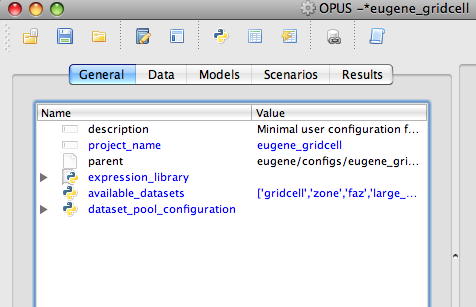
\includegraphics[scale=0.6]{part-gui/images/general-tab.png}
\end{center}
\caption{The General Tab}
\label{fig:general}
\end{figure}

